Throughout this chapter, $T=5$ is the number of tasks and experts, $i$ indexes experts, $t$ is the task of an input, $\ell\in\{1,\dots,12\}$ indexes encoder layers, and $j$ indexes the $N$ tokens of an input. The method is described as implemented in this study.

\section{BERT Encoder and Shared Backbone}

BERT~\cite{devlin2019bert} is an encoder-only Transformer~\cite{vaswani2017attention}. This study uses \texttt{bert-base-uncased}, with 12 encoder layers, hidden size $d=768$, 12 attention heads and an MLP size of 3072, for 109.5M parameters per expert including the head. Figure~\ref{fig:bert} shows the structure. Tokens are mapped to the sum of a token, a segment and a position embedding, followed by layer normalisation~\cite{ba2016layernorm}. Each encoder layer then has two sub-layers. Self-attention gives each token a state that reflects its whole context, relating queries $Q$ to keys $K$ of dimension $d_k$ and values $V$:
\begin{equation}
\mathrm{Attention}(Q,K,V)=\mathrm{softmax}\!\left(\frac{QK^{\top}}{\sqrt{d_k}}\right)V .
\label{eq:attention}
\end{equation}
The second sub-layer is a position-wise feed-forward network, called the \emph{MLP block} here:
\begin{equation}
\mathrm{MLP}(h)=W_2\,\mathrm{GELU}(W_1h+b_1)+b_2 ,
\label{eq:ffn}
\end{equation}
where $h$ is a token state, GELU is the activation of Hendrycks and Gimpel~\cite{hendrycks2016gelu}, and $(W_1,b_1)$ and $(W_2,b_2)$ are the first and second linear layers of the block, called fc1 and fc2. Each sub-layer is wrapped as $h'=\mathrm{LayerNorm}\big(h+\mathrm{Sublayer}(h)\big)$. For classification, the final \texttt{[CLS]} state passes through the pooler, a dense layer with $\tanh$, and then a task-specific head $g_t$ made of dropout and a linear layer with two outputs. All experts start from the same weights and share this structure, so their weights can be subtracted and added position by position.

\begin{figure}[htbp]
  \centering
  \resizebox{.82\linewidth}{!}{% BERT encoder as traced from the code; same diagram as slide 6 of the presentation.
\begin{tikzpicture}[x=1cm,y=1cm]
  \tikzset{every node/.append style={font=\figfont}}
  \node[plain] (x) at (.35,0) {Tokens $x$\\ \texttt{[CLS]} $A$ \texttt{[SEP]}\\ (+ $B$ \texttt{[SEP]})};
  \node[frz,minimum width=2.35cm] (emb) at (3.65,0) {Embeddings\\ token + segment + position, LayerNorm};
  \node[frz,minimum width=2.3cm,very thick] (enc) at (7.4,0) {\textbf{Encoder layer} $\ell$\\ repeated $\times 12$};
  \node[frz,minimum width=1.75cm] (pool) at (9.85,0) {Pooler\\ {[CLS]}: dense, tanh};
  \node[frz,minimum width=1.6cm] (head) at (12.0,0) {Head $g_t$\\ dropout, linear};
  \node[plain] (out) at (13.55,0) {Logits\\ $\to\hat y$};
  \foreach \a/\b in {x/emb,emb/enc,enc/pool,pool/head,head/out} \draw[flow] (\a) -- (\b);
  \node[plain] (in) at (.55,-1.75) {$h$};
  \node[frz,minimum width=1.9cm] (att) at (2.25,-1.75) {Multi-head\\ self-attention};
  \node[frz,minimum width=.95cm] (an1) at (4.2,-1.75) {Add\\ \&Norm};
  \node[mix,minimum width=1.2cm] (fc1) at (6.05,-1.75) {Linear fc1\\ $W_1,b_1$};
  \node[frz,minimum width=.85cm] (act) at (7.5,-1.75) {GELU};
  \node[mix,minimum width=1.2cm] (fc2) at (8.95,-1.75) {Linear fc2\\ $W_2,b_2$};
  \node[frz,minimum width=.95cm] (an2) at (10.85,-1.75) {Add\\ \&Norm};
  \node[plain] (outh) at (12.4,-1.75) {$h'$};
  \foreach \a/\b in {in/att,att/an1,an1/fc1,fc1/act,act/fc2,fc2/an2,an2/outh} \draw[flow] (\a) -- (\b);
  \coordinate (r1) at ($(in.east)!.45!(att.west)$);
  \coordinate (r2) at ($(an1.east)!.45!(fc1.west)$);
  \draw[flow] (r1) -- ++(0,.62) -| (an1.north);
  \draw[flow] (r2) -- ++(0,.62) -| (an2.north);
  \begin{scope}[on background layer]
    \node[group,draw=BurntOrange,thick,fit=(fc1)(act)(fc2)] (mlp) {};
    \coordinate (ltop) at ($(r1)+(0,.62)$);
    \coordinate (lbot) at ($(mlp.south)+(0,-.32)$);
    \node[group,inner sep=5pt,fit=(in)(outh)(att)(an2)(ltop)(lbot)] (lay) {};
  \end{scope}
  \draw[black!45,dotted,thick] (enc.south west) -- (lay.north west);
  \draw[black!45,dotted,thick] (enc.south east) -- (lay.north east);
  \node[font=\figfont\bfseries,text=BurntOrange!85!black,anchor=north] at (mlp.south) {MLP block: its linear layers are upscaled by WEMoE};
\end{tikzpicture}
}
  \caption{BERT encoder as used in this study, from the input tokens to the logits (top), with one encoder layer enlarged (bottom). Dropout layers are not drawn.}
  \label{fig:bert}
\end{figure}

\section[WEMoE Architecture: Static and Input-Conditioned Merging]{WEMoE Architecture: Static and\\ Input-Conditioned Merging}

WEMoE splits the parameters into two groups. In the design of Tang et al.~\cite{tang2024wemoe}, shown in Figure~\ref{fig:overview}, attention and layer normalisation are merged statically, and each MLP is ``upscaled'' to a Weight-Ensembling MoE module, meaning that its weights become input-conditioned. Their vision Transformers normalise before each sub-layer. BERT normalises after it, so Figure~\ref{fig:arch} shows the same principle as implemented on BERT. Here the static group is every weight of the encoder outside the upscaled layers, including embeddings and pooler. Table~\ref{tab:components} lists the components, where $W_0^{\ell}$ and $\tau_i^{\ell}$ are the parts of $\theta_0$ and $\tau_i$ that belong to the MLP of layer $\ell$, $\lambda$ is the scaling factor of Section~\ref{sec:ta} and $r^{\ell}$ is the router of Section~\ref{sec:router}. The router sees only token states and does not receive the task identifier, which selects the head alone.

\begin{figure}[htbp]
  \centering
  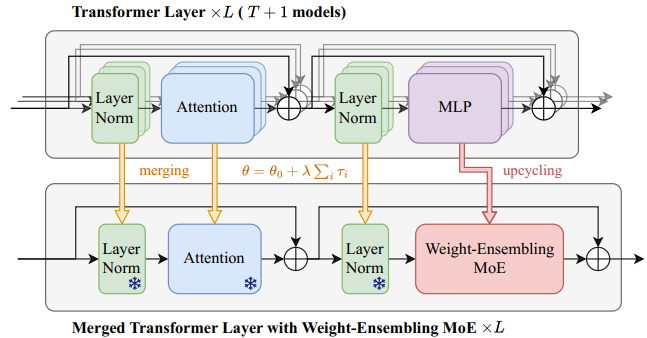
\includegraphics[width=.38\linewidth]{arch_wemoe_overview.png}
  \caption{Original WEMoE design on a pre-norm vision Transformer, from Tang et al.~\cite{tang2024wemoe}. Top: the fine-tuned and pre-trained models. Bottom: the merged layer. Frozen parts carry a snowflake mark.}
  \label{fig:overview}
\end{figure}

\begin{figure}[htbp]
  \centering
  \resizebox{.76\linewidth}{!}{\begin{tikzpicture}[x=1cm,y=1cm]
  \node[plain] (in) at (.35,0) {Tokens $x$\\task id $t$};
  \node[frz,minimum width=1.2cm] (emb) at (1.72,0) {Embed-\\dings};
  \node[frz,minimum width=1.7cm] (att) at (3.75,0) {Multi-head\\attention\\+ Add\&Norm};
  \node[mix,minimum width=1.2cm] (fc1) at (6.0,0) {fc1\\$W^{\ell}_1(x)$};
  \node[frz,minimum width=.9cm] (act) at (7.45,0) {GELU};
  \node[mix,minimum width=1.2cm] (fc2) at (8.9,0) {fc2\\$W^{\ell}_2(x)$};
  \node[frz,minimum width=1.1cm] (nrm) at (10.5,0) {Add\\\&Norm};
  \node[frz,minimum width=1.1cm] (pool) at (12.45,0) {Pooler\\(TA)};
  \node[frz,minimum width=1.0cm] (head) at (14.0,0) {Head\\$g_t$};
  \node[plain] (out) at (15.75,0) {Logits\\$\to\hat y$};
  \foreach \a/\b in {in/emb,emb/att,att/fc1,fc1/act,act/fc2,fc2/nrm,nrm/pool,pool/head,head/out}
    \draw[flow] (\a) -- (\b);
  \node[frz,minimum width=3.4cm] (ta) at (2.35,1.9) {Task Arithmetic, $\lambda=0.3$\\$\theta=\theta_0+\lambda\sum_i\tau_i$};
  \node[frz,minimum width=4.2cm] (dict) at (7.35,1.9) {Dictionary per upscaled module\\$W_0^{\ell},\ \tau^{\ell}_{\mathrm{MRPC}},\dots,\tau^{\ell}_{\mathrm{QNLI}}$};
  \node[frz,minimum width=4.6cm] (src) at (13.3,1.9) {Pre-trained $\theta_0$ + five experts $\theta_i$\\(each expert also supplies a head $g_i$)};
  \draw[dict] (ta.south -| emb) -- (emb);
  \draw[dict] (ta.south -| att) -- (att);
  \draw[dict] (dict.south -| fc1) -- (fc1);
  \draw[dict] (dict.south -| fc2) -- (fc2);
  \draw[dict] (src.west) -- (dict.east);
  \draw[dict] (dict.west) -- (ta.east);
  \draw[dict] (src.south -| head) -- (head);
  \node[trn,minimum width=3.2cm] (rt) at (7.45,-1.6) {Router $r^{\ell}$ (one per layer)};
  \coordinate (tap) at ($(att.east)!.45!(fc1.west)$);
  \draw[gate] (tap) |- (rt.west);
  \node[note,anchor=east] at ($(tap |- rt.west)+(-.05,0)$) {token states $h_i$};
  \draw[gate] (rt.north -| fc1) -- (fc1.south);
  \draw[gate] (rt.north -| fc2) -- (fc2.south);
  \node[note,anchor=west] (gw) at (9.5,-1.6) {gating weights $w^{\ell}(x)\in\mathbb{R}^{T}$,\\shared by fc1 and fc2};
  \begin{scope}[on background layer]
    \node[group,fit=(att)(nrm)(rt)(gw)] (g) {};
  \end{scope}
  \node[note,anchor=north east] at (g.south east) {encoder layer $\ell$, repeated $\times 12$};
\end{tikzpicture}
}\\[2pt]
  \figlegend
  \caption{Merged WEMoE model as implemented. In the full scope both fc1 and fc2 are input-conditioned. In the intermediate-only scope fc2 is static and uses Task Arithmetic.}
  \label{fig:arch}
\end{figure}

\begin{table}[htbp]
  \centering\tablestyle
  \caption{Components of the merged model in the default full-MLP variant.}
  \label{tab:components}
  \begin{tabularx}{\linewidth}{l X c}
    \toprule
    Component & Origin & During FSFT\\
    \midrule
    Embeddings, attention, layer norm, pooler & Task Arithmetic with $\lambda$ chosen on dev & Frozen\\
    MLP base weights $W_0^{\ell}$ & Pre-trained model & Frozen\\
    MLP task vectors $\tau_i^{\ell}$ & Experts minus pre-trained model & Frozen\\
    Classification heads $g_t$ & One from each expert & Frozen\\
    Routers $r^{\ell}$ & New, one per encoder layer & \textbf{Trained}\\
    \bottomrule
  \end{tabularx}
\end{table}

The split sets the storage cost. A static part is stored once. Each upscaled layer must keep its pre-trained weights and one task vector per expert, which is $T+1$ copies of that layer, and the routers add their own parameters $\phi$:
\begin{equation}
|\theta_{\mathrm{static}}|+(T+1)\,|\theta_{\mathrm{MLP}}|+|\phi|+|\mathrm{heads}|,
\label{eq:storage}
\end{equation}
where $\theta_{\mathrm{MLP}}$ denotes the upscaled layers. We evaluate two scopes: \emph{full}, which upscales fc1 and fc2, and \emph{intermediate-only}, which upscales fc1 alone. The task vectors account for most of the stored parameters of the full scope (Table~\ref{tab:storage}), so the saving depends strongly on this choice. Tang et al.\ base the choice of the MLP on their observation for CLIP-ViT models that attention weights stay closer in direction to the pre-trained model than MLP weights do. We did not repeat that measurement on BERT, so the choice is inherited and not independently justified here.

\section{Task Arithmetic and Task Vectors}
\label{sec:ta}

A task vector (Equation~\ref{eq:task-vector}) records what fine-tuning changed for a task. Task Arithmetic~\cite{ilharco2023task} adds the vectors back to the base with one scaling factor $\lambda$:
\begin{equation}
\theta=\theta_0+\lambda\sum_{i=1}^{T}\tau_i .
\label{eq:ta}
\end{equation}
Simple Averaging is the special case $\lambda=1/T$, which equals the mean of the expert weights. A small $\lambda$ stays near the pre-trained model, and a large one applies the updates more strongly, including any conflicts among them. We select $\lambda$ by grid search on the mean development score (Section~\ref{sec:merging}). The method is simple and adds no parameters, but its result is the same for every input.

\section{Router and Input-Conditioned MLP}
\label{sec:router}

Each encoder layer has its own router $r^{\ell}$ (Figure~\ref{fig:router}). Its input is the sequence of token states $h^{\ell}_j\in\mathbb{R}^{d}$ that leave the first Add\&Norm of the layer. The router has two linear layers with a ReLU and is applied to every token:
\begin{equation}
r^{\ell}(h)=A^{\ell}_2\,\mathrm{ReLU}\big(A^{\ell}_1h+c^{\ell}_1\big)+c^{\ell}_2,
\label{eq:router}
\end{equation}
with $A^{\ell}_1\in\mathbb{R}^{d\times d}$ and $A^{\ell}_2\in\mathbb{R}^{T\times d}$. The twelve routers hold $12\,(d^2+d+Td+T)=7{,}133{,}244$ trainable parameters. Token outputs are averaged over non-padding positions, using the attention mask $m_j\in\{0,1\}$, to give one vector per input, so that padding does not affect routing:
\begin{equation}
w^{\ell}(x)=\frac{\sum_j m_j\,r^{\ell}(h^{\ell}_j)}{\sum_j m_j}\in\mathbb{R}^{T}.
\label{eq:gating}
\end{equation}
For an input $x$, each upscaled linear layer is rebuilt from its pre-trained weights and its part of the task vectors, and its bias is rebuilt in the same way:
\begin{equation}
W^{\ell}(x)=W_0^{\ell}+\sum_{i=1}^{T}w_i^{\ell}(x)\,\tau_i^{\ell},\qquad
b^{\ell}(x)=b_0^{\ell}+\sum_{i=1}^{T}w_i^{\ell}(x)\,\tau_i^{\ell,b}.
\label{eq:we}
\end{equation}
Both linear layers of a block share the same $w^{\ell}(x)$. The prediction uses the head $g_t$ of the known task, where $\bar\theta$ denotes the statically merged weights:
\begin{equation}
p(y\mid x,t)=\mathrm{softmax}\Big(g_t\big(\mathrm{pool}(\mathrm{BERT}(x;\bar\theta,\{W^{\ell}(x)\}))\big)\Big),\quad
\hat y=\arg\max_{y}\,p(y\mid x,t).
\label{eq:prediction}
\end{equation}

\begin{figure}[htbp]
  \centering
  \begin{minipage}[c]{.25\linewidth}\centering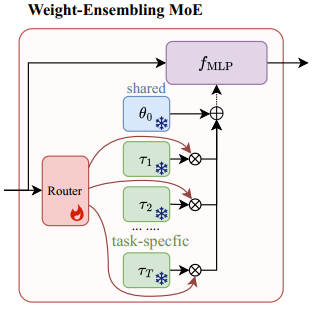
\includegraphics[width=\linewidth]{arch_wemoe_module.png}\end{minipage}\hfill
  \begin{minipage}[c]{.72\linewidth}\centering\resizebox{\linewidth}{!}{\begin{tikzpicture}[x=1cm,y=1cm]
  \node[plain] (h) at (0,0) {$h^{\ell}_i\in\mathbb{R}^{768}$\\per token};
  \node[trn,minimum width=1.9cm] (a1) at (2.5,0) {Linear $A_1,c_1$\\$768\to768$};
  \node[trn,minimum width=1.0cm] (re) at (4.45,0) {ReLU};
  \node[trn,minimum width=1.9cm] (a2) at (6.4,0) {Linear $A_2,c_2$\\$768\to5$};
  \node[frz,minimum width=1.6cm] (mm) at (9.1,0) {Masked\\mean};
  \node[plain] (w) at (11.5,0) {$w^{\ell}(x)\in\mathbb{R}^{5}$\\one per input};
  \foreach \a/\b in {h/a1,a1/re,re/a2,a2/mm,mm/w} \draw[gate] (\a) -- (\b);
  \node[dat,minimum width=2.1cm] (m) at (9.1,-1.45) {Attention mask $m_i$};
  \draw[flow] (m) -- (mm);
  \node[note,text width=7.2cm,anchor=north] at (3.6,-.75) {Initialisation: $A_1,A_2\sim\mathcal{N}(0,0.01^2)$, $c_1=0$, $c_2=\lambda$, so that $w_e^{\ell}(x)\approx\lambda$ and the model starts close to Task Arithmetic. No softmax and no top-$k$ selection are applied.};
\end{tikzpicture}
}\end{minipage}
  \caption{Left: the WEMoE module of Tang et al.~\cite{tang2024wemoe}. Right: router of layer $\ell$ as implemented, applied per token and averaged over non-padding tokens.}
  \label{fig:router}
\end{figure}

The router's values are \emph{unnormalised}. With no softmax and no top-$k$ selection, a value can exceed 1 or be negative, so a router can amplify or subtract a task vector, and the combination is neither convex nor sparse. Linear weights are initialised from $\mathcal{N}(0,0.01^2)$ with $c^{\ell}_1=0$ and $c^{\ell}_2=\lambda$, so $w^{\ell}_i(x)\approx\lambda$ at the start and the model begins close to Task Arithmetic. Unit tests on small random models confirm that constant routing equals Task Arithmetic, that padding does not affect routing and that only the routers receive gradients.

\section{Few-Shot Fine-Tuning (FSFT) Objective}
\label{sec:fsft}

The routers are trained with Few-Shot Fine-Tuning: cross-entropy on a small labelled set, summed over the tasks. For each task, $k$ examples $D_t^{(k)}$ are drawn from a reserved pool, and for a fixed seed a smaller $k$ gives a subset of a larger one. At each step, one mini-batch $B_t$ is drawn per task, and the objective is
\begin{equation}
\min_{\phi}\ \sum_{t=1}^{T}\ \frac{1}{|B_t|}\sum_{(x,y)\in B_t}-\log p_{\phi}(y\mid x,t),
\qquad B_t\subset D_t^{(k)},\ \ |D_t^{(k)}|=k ,
\label{eq:fsft}
\end{equation}
where $p_\phi$ is the distribution of Equation~\eqref{eq:prediction}. Everything except $\phi$ stays frozen, and dropout is disabled. The mean development score is evaluated before training and every 50 steps, and the router state of the best step is restored at the end. A run whose best step is 0 therefore reports the untrained router.

Table~\ref{tab:comparison} separates the original method from this study. The largest difference is the objective. Tang et al.\ minimise prediction entropy on unlabelled test data, which is test-time adaptation, and this objective is not used here. FSFT instead uses labelled training examples and never touches the reporting split. The results of the two studies are therefore not directly comparable.

\begin{table}[htbp]
  \centering\tablestyle
  \caption{The original WEMoE study of Tang et al.~\cite{tang2024wemoe} and this study.}
  \label{tab:comparison}
  \begin{tabularx}{\linewidth}{>{\bfseries\raggedright\arraybackslash}p{2.9cm} *{2}{>{\raggedright\arraybackslash}X}}
    \toprule
    Aspect & Tang et al. & This study\\
    \midrule
    Backbone, tasks & CLIP-ViT vision models; eight image classification tasks & BERT-base; five binary GLUE tasks\\
    Router training & Test-time adaptation: entropy on unlabelled test data & FSFT: cross-entropy on $k$ labelled examples per task\\
    Routing input & Mean over tokens & Mean over non-padding tokens\\
    Upscaled modules & Transformer MLPs & Full MLP; intermediate-only as an ablation\\
    \bottomrule
  \end{tabularx}
\end{table}
